\documentclass[al, 27pt, plainboxedsections, landscape]{sciposter}
\usepackage{multicol}
\usepackage{sectionbox}
\usepackage[demo]{graphicx}
\usepackage{subfig}
\usepackage[numbers, longnamesfirst, sort]{natbib}

\definecolor{darkgreen}{rgb}{0,0.4,0}

\newcommand{\tb}[1]{\textcolor{blue}{#1}}
\newcommand{\tre}[1]{\textcolor{red}{#1}}
\newcommand{\tgrey}[1]{\textcolor{grey}{#1}}
\newcommand{\tgr}[1]{\textcolor{darkgreen}{#1}}
\newcommand{\tye}[1]{\textcolor{yellow}{#1}}
\newcommand{\cya}[1]{\textcolor{cyan}{#1}}
\newcommand{\cnt}[1]{{\tt \textcolor{cyan}{#1}}}

\title{Computing Kantorovich-Wasserstein Distances on $d$-dimensional histograms using $(d+1)-$partite graphs}
\leftlogo[1.3]{images/logo_unipv}

\author{Gennaro Auricchio$^{a}$, Federico Bassetti$^b$, Stefano Gualandi$^a$, Marco Veneroni$^a$}
\institute{$^{(a)}$ Universit\`{a} degli Studi di Pavia, Dipartimento di Matematica ``F.Casorati'',$\quad ^{(b)}$ Politecnico di Milano, Dipartimento di Ingegneria Matematica}
\email{gennaro.auricchio01@universitadipavia.it,stefano.gualandi@unipv.it,marco.veneroni@unipv.it,federico.bassetti@polimi.it}

\begin{document}
\maketitle
\begin{multicols}{3}
	
	\begin{abstract}	
	\large{	
		\begin{itemize}		
			\item[] \cya{{\bf TASK}: To compute the distance between two $d$-dimensional histograms having $n$ bins. For instance, images are 2-dimensional histograms with $n$ bins (pixels)}
			\item[] \tb{{\bf PROBLEM}: The mathematical tool used to compute this distance requires the solution of an optimization problem with up to $n^2$ variables}
			\item[] \tre{{\bf IDEA}: To exploit the structure of the cost function in order to reduce the number of variables of the optimization problem}
		\end{itemize}}
	\end{abstract}
	
\section{Kantorovich-Wasserstein distance} 

\begin{itemize}
\item[] 
The \tre{Kantorovich-Wasserstein distance}
is a metric  between
probability distributions or  \tgr{d-dimensional histograms}.
%\item[] Among various applications, 
%this metric is used in  \tgr{image processing}, by coding  
% images as $2D$ normalized histograms. 
\end{itemize}

%The optimal transport is a tool that is nowadays used to compute distances between images. 
%For example the $W_2$ distance is used in image processing, but it is still a problem to compute $W_2$ efficiently. 




% The optimal transport is a tool that is nowadays used to compute distances between images. 
%For example the $W_2$ distance is used in image processing, but it is still a problem to compute $W_2$ efficiently. 

 \begin{figure}
     \centering
     {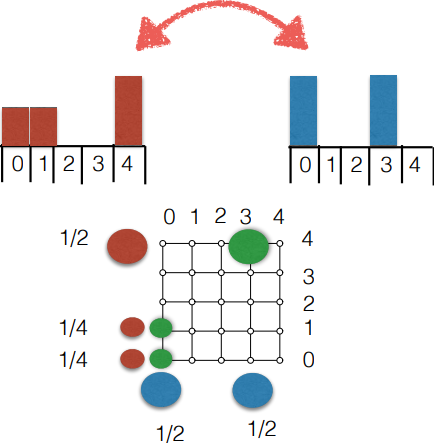
\includegraphics[width=0.35\columnwidth]{images/intro_disc}\label{<figure1>}}
	 \hspace{0.09\columnwidth}
     {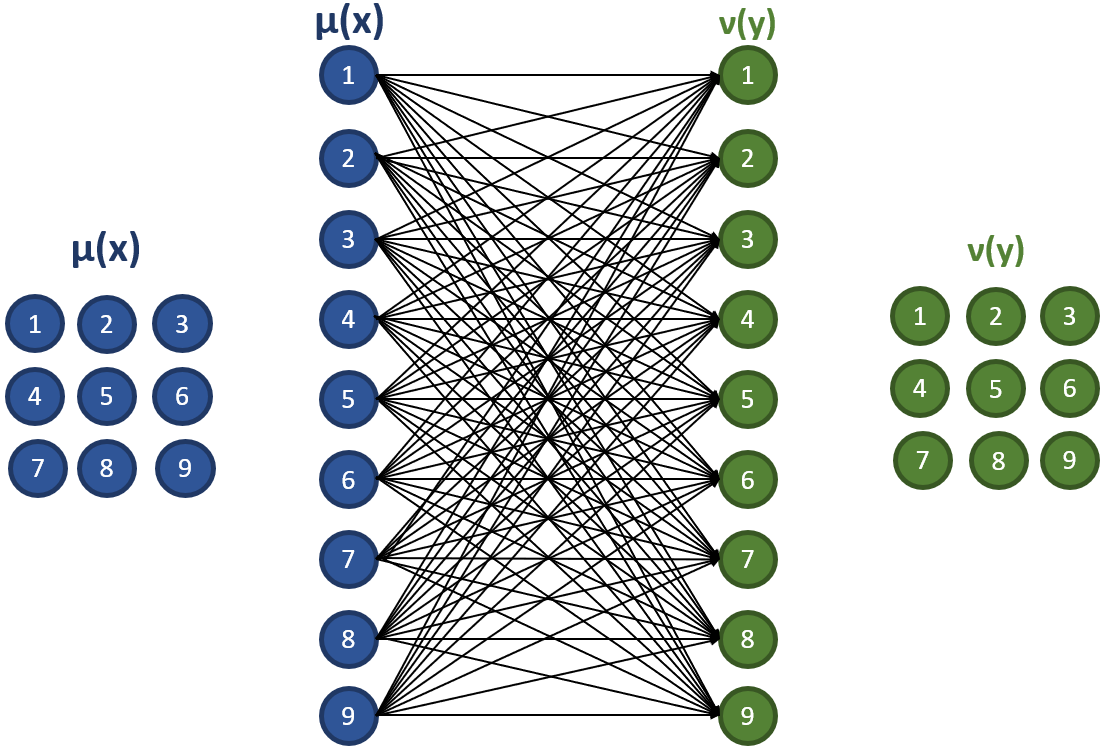
\includegraphics[width=0.5\columnwidth]{images/fig3}\label{<figure2>}}
     \caption{Left: transport map $\pi$  (green dots) between $1D $-histograms (red and blue dots) with $n=5$ bins. 
     Right:
     bipartite graph associated to  constrained optimization problem used to compute the
     Kantorovich-Wasserstein distance for $2D $-histograms with $n=9$ bins}
     \label{steady_state}
\end{figure}



%As shown in Figure \ref{steady_state} (left) for $1D$-histograms, 
The idea of 
the Kantorovich-Wasserstein distance is to find 
 the \tb{optimal} way to map a probability $\mu$ to a probability $\nu$ where   \tgr{moving a unit mass from $x$ to $y$ costs $c_{x,y}$}.
 Figure \ref{steady_state} (left).
 
%For the sake of clarity and brevity we will work with $2D$ grids.\newline
	
%We want to find the optimal way to map a probability $\mu$ to a probability $\nu$ where moving a unit mass from $x$ to $y$ 
Whenever the cost  is \tre{$c_{x,y}=\|x-y\|_2^2$}, % $c_{x,y}=(x_1-y_1)^2 + (x_2-y_2)^2$, 
one gets the \tre{Wasserstein distance of order 2}
\tre{
\[
W_2(\mu,\nu) := \min \sum_{x}\sum_{y}c_{x,y} \pi_{x,y}
\]}
where the minimum is over all the probability measures $\pi$ with \tgr{marginals $\nu$ and $\mu$},  i.e. 
%$\sum_{x}\pi_{x,y}=\nu_y$ and $\sum_{y}\pi_{x,y}= \mu_x$.
\[
\sum_{x}\pi_{x,y}=\nu_y, \;\;\;\;\; \emph{and}  \;\;\;\;\; \sum_{y}\pi_{x,y}= \mu_x.
\]



The computation of  $W_2$ distances between  histograms with $n$ bins
requires the solution of a \tre{constrained optimization problem}.
%, which is usually
%\tgr{computationally too heavy} even for moderate size $n$. 


Indeed, the standard approach to compute $W_2$ distances between $2D$ histograms with $n$ bins is to solve 
the corresponding 
 \tb{uncapacitated min cost flow problem} \cite{GG1} on a  \tre{bipartite graph}, with  \tre{$2n$ nodes} 
 (2 times the number of bins) and  \tre{$n^2$ arcs} (one for all the possible costs $c_{x,y}$).
 See Figure  \ref{steady_state} (right). 
 \newline
 
The solution of this problem requires $O(n^3 \log (n))$ time, which 
for large $n$ is \tgr{computationally too heavy}.
 

\section{Our contribution}

In \cite{GG2}  we  propose a novel approach for computing 
the $W_2$ distance 
 that exploits \tb{the structure of the cost} function to \tre{reduce the number of arcs}. 

\begin{figure}[!t]
	\centering
	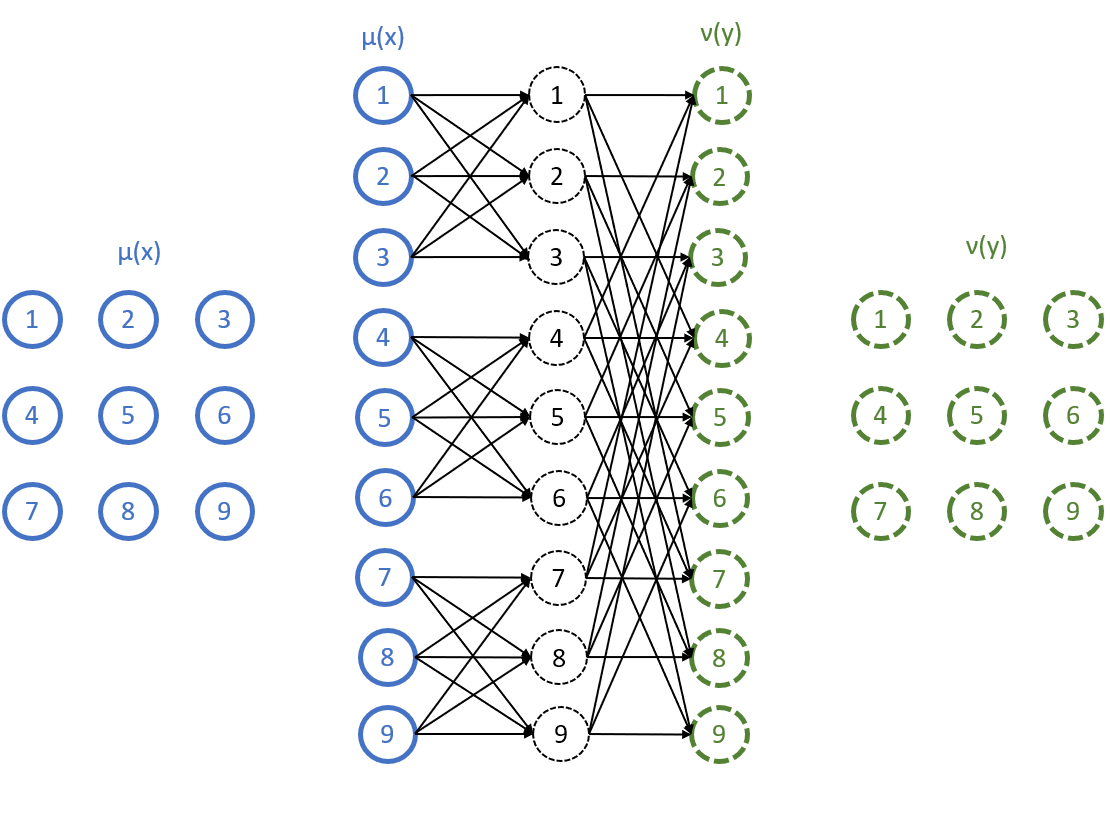
\includegraphics[width=0.75\columnwidth]{images/fig6}
	 \caption{$3-$partite graph reformulation for the computation of $W_2$}
     \label{Figure2}
\end{figure}


Since the cost function is \tb{separable}, 
$c_{x,y}=(x_1-y_1)^2 + (x_2-y_2)^2$, it
can be computed as the \tb{concatenation} of  the costs  along the \tb{two main directions}:
$(x_1,x_2) \to (y_1,x_2)$ and $(y_1,x_2) \to (y_1,y_2)$. See Figure \ref{Figure2}. 
\newline

{\large \tre{{\bf CONTRIBUTION:}}
\textit{
We prove that 
 the $W_2$ distance
between \tre{$d$-dimensional}  histograms can 
be computed as a flow problem 
on a  \tre{$(d+1)$-partite graph},  with   $(d+1)n$ nodes
  and  \tre{$dn^{1+\frac{1}{d}}$ arcs}. }}
% See Figure \ref{Figure2} (right).



\begin{itemize}
	\item Our method requires  \tre{$dn^{1+\frac{1}{d}}$ arcs} while the standard bipartite graph method requires $n^2$.
	\item The method can be adapted  to any \tb{cost function} that is \tb{separable}, \emph{i.e.} can be written as a sum of independent contributions.
	\item  The method provides an \tre{exact solution}. 
	%and still  outperforms  all known exact and approximated methods.
\end{itemize}

\section{Numerical Results}
As problem instances, we use the gray scale images proposed by
the DOTMark benchmark, and a set of $d$-dimensional histograms obtained by biomedical data
measured by flow cytometry.

\begin{table}
\caption{Comparison on Flow Cytometry data with increasing value of $d$.}
	\label{tab:3}
\centering
{\renewcommand{\arraystretch}{1.2}
\begin{tabular}{l@{\hskip 0.4in}l@{\hskip 0.4in}r@{\hskip 0.4in}rrr@{\hskip 0.4in}rr@{\hskip 0.4in}r}
     \multicolumn{3}{c}{} & \multicolumn{3}{c}{Bipartite Graph} & \multicolumn{3}{c}{$(d+1)$-partite Graph} \\
	 \hline
N & $d$ & $n$ & $|V|$ & $|A|$ & Runtime & $|V|$ & $|A|$ & Runtime  \\
\hline
$16$ & 2 & 256 & 512 & 65\,536 & 0.024 (0.01) & 768 & 8\,192 & {\bf 0.003 (0.00)} \\
& 3 & 4\,096 & 8\,192 & 16\,777\,216& 38.2 (14.0)   & 16\,384 & 196\,608& {\bf 0.12 (0.02)}  \\
& 4 & 65\,536 & \multicolumn{3}{c}{{\it out-of-memory}} & 327\,680 & 4\,194\,304& {\bf 4.8 (0.84)} \\
 \hline\noalign{\smallskip}
$32$ & 2 & 1\,024 & 2\,048 & 1\,048\,756 & 0.71 (0.14) & 3072 & 65\,536& {\bf 0.04 (0.01)} \\
& 3 & 32\,768& \multicolumn{3}{c}{{\it out-of-memory}}   & 131\,072 & 3\,145\,728& {\bf 5.23 (0.69)}  \\
 \hline\noalign{\smallskip}
 \end{tabular}}
\end{table}

\begin{figure}[!t]
\centering
{\renewcommand{\arraystretch}{0.7}
\setlength{\tabcolsep}{0.1em}
\begin{tabular}{cccccccccc}
  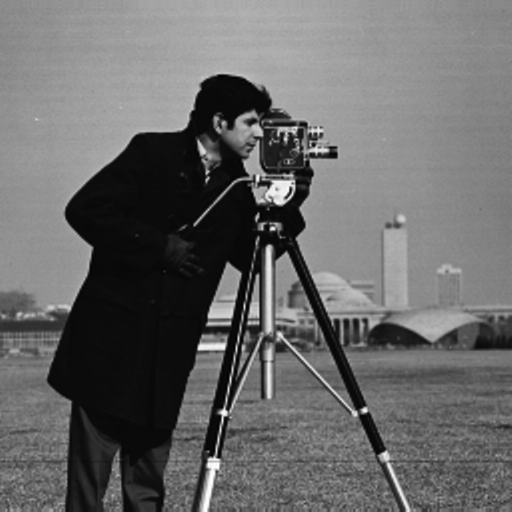
\includegraphics[width=0.095\linewidth]{images/classic512_1001}  & 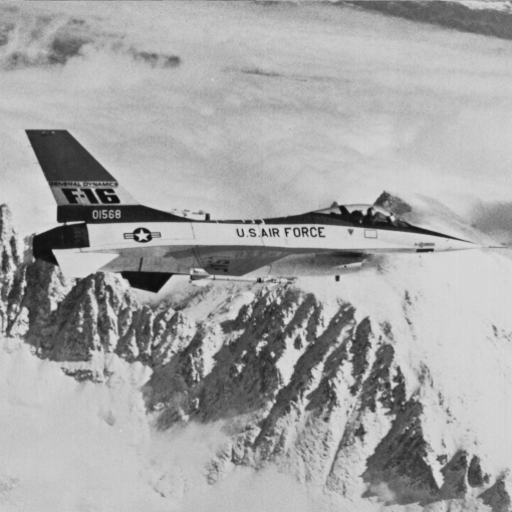
\includegraphics[width=0.095\linewidth]{images/classic512_1002} &
  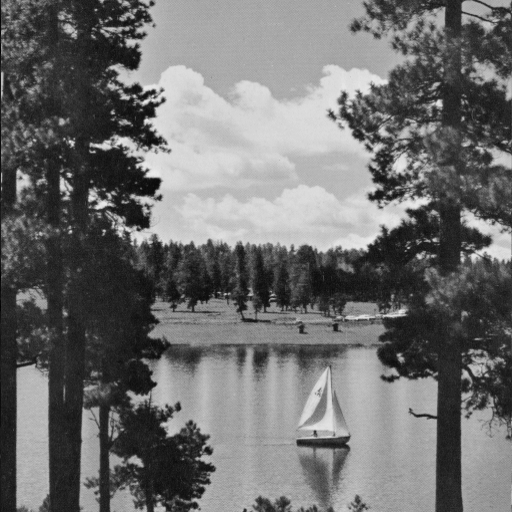
\includegraphics[width=0.095\linewidth]{images/classic512_1003} & 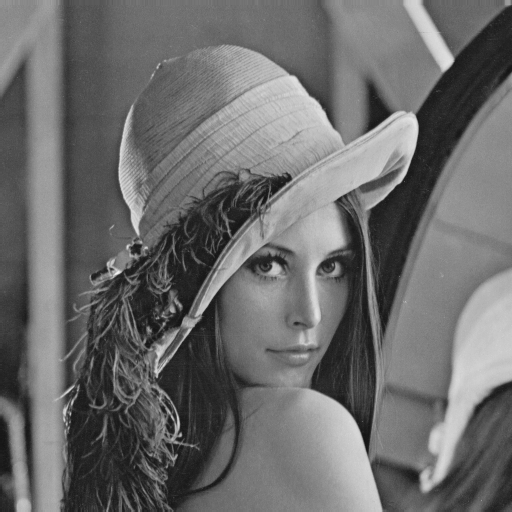
\includegraphics[width=0.095\linewidth]{images/classic512_1004} &
  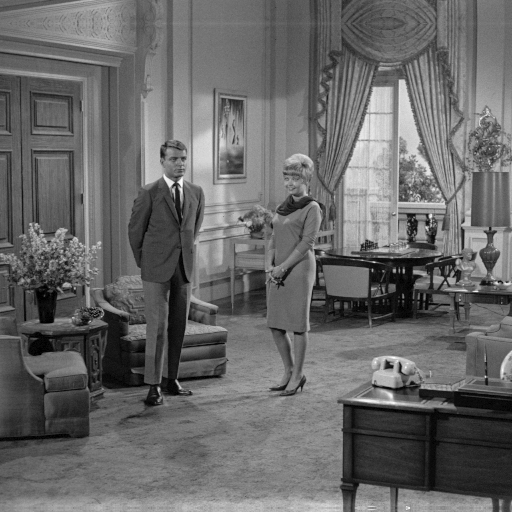
\includegraphics[width=0.095\linewidth]{images/classic512_1005} &
  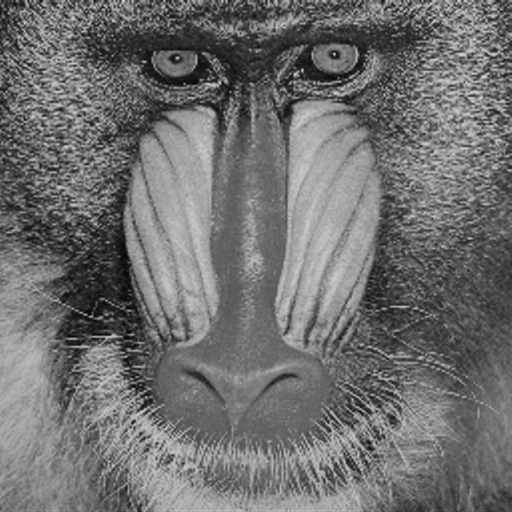
\includegraphics[width=0.095\linewidth]{images/classic512_1006}  & 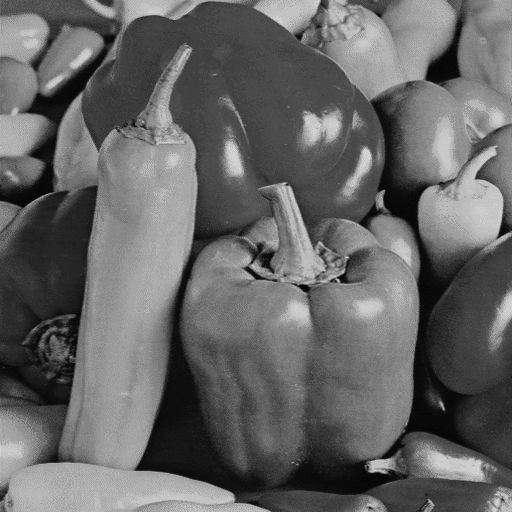
\includegraphics[width=0.095\linewidth]{images/classic512_1007} &
  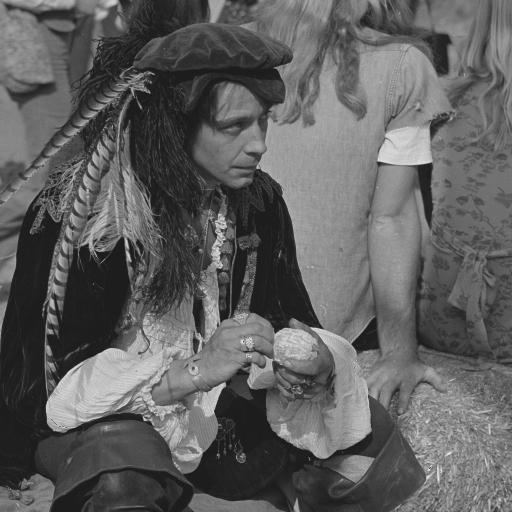
\includegraphics[width=0.095\linewidth]{images/classic512_1008} & 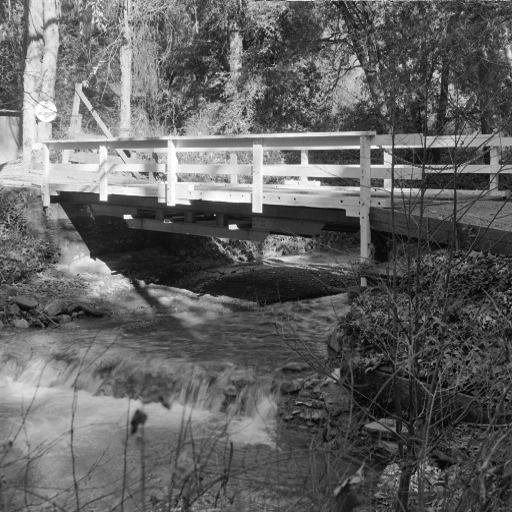
\includegraphics[width=0.095\linewidth]{images/classic512_1009} &
  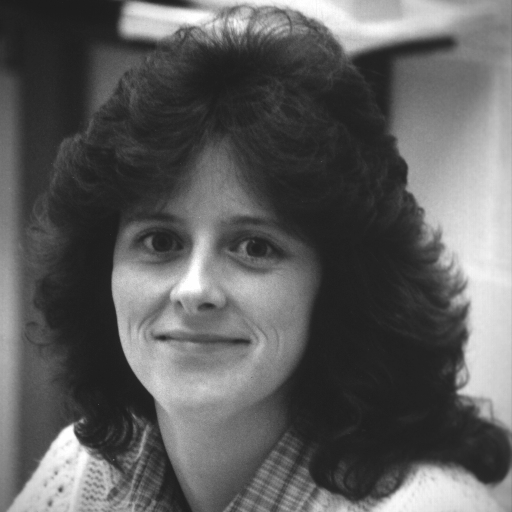
\includegraphics[width=0.095\linewidth]{images/classic512_1010} \\  
  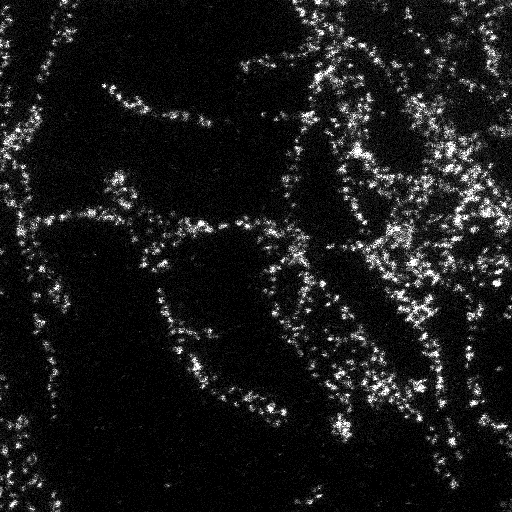
\includegraphics[width=0.095\linewidth]{images/micro512_1001}  & 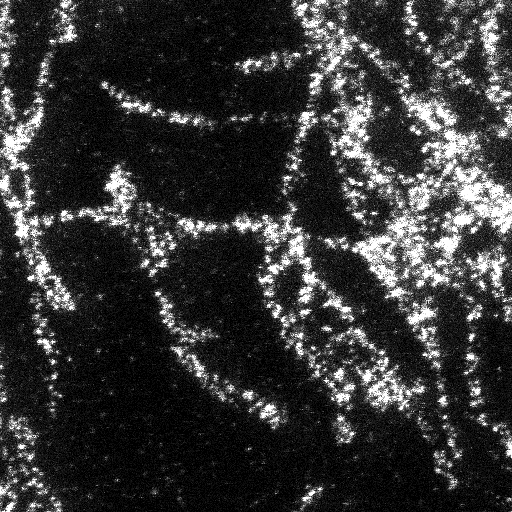
\includegraphics[width=0.095\linewidth]{images/micro512_1002} &
  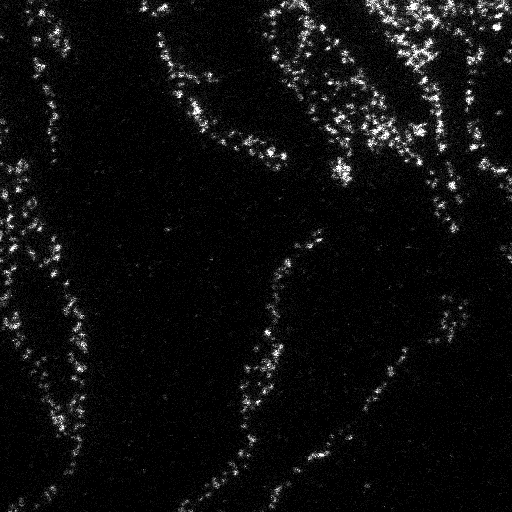
\includegraphics[width=0.095\linewidth]{images/micro512_1003} & 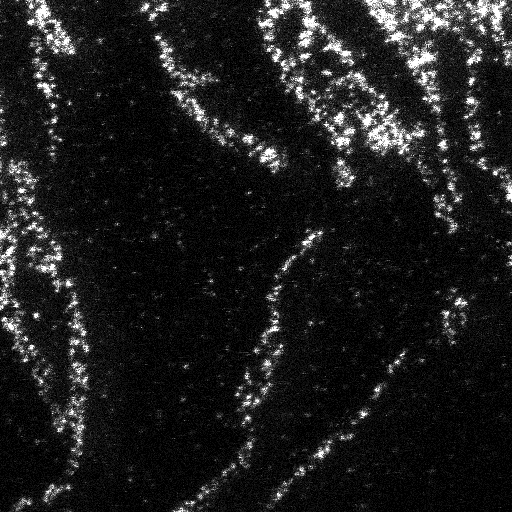
\includegraphics[width=0.095\linewidth]{images/micro512_1004} &
  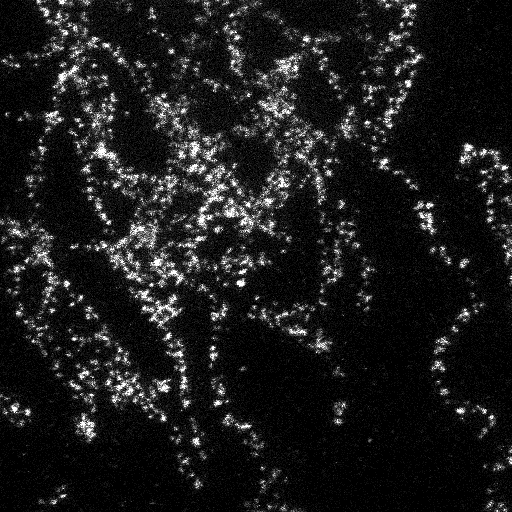
\includegraphics[width=0.095\linewidth]{images/micro512_1005} &
  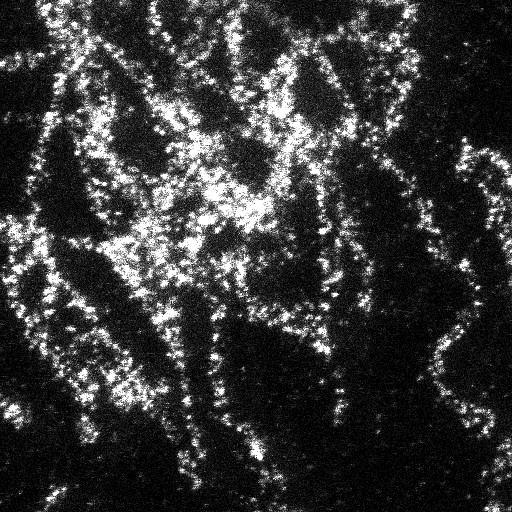
\includegraphics[width=0.095\linewidth]{images/micro512_1006}  & 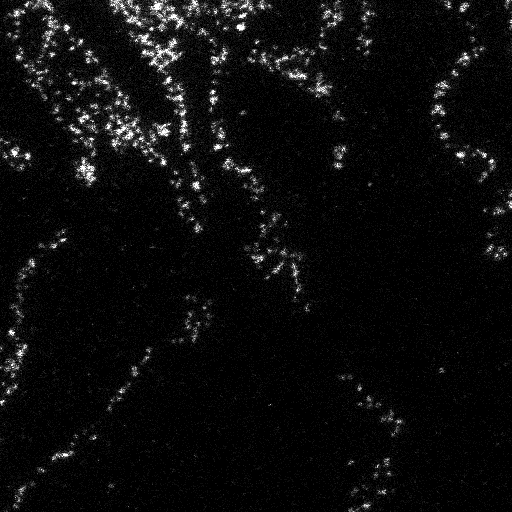
\includegraphics[width=0.095\linewidth]{images/micro512_1007} &
  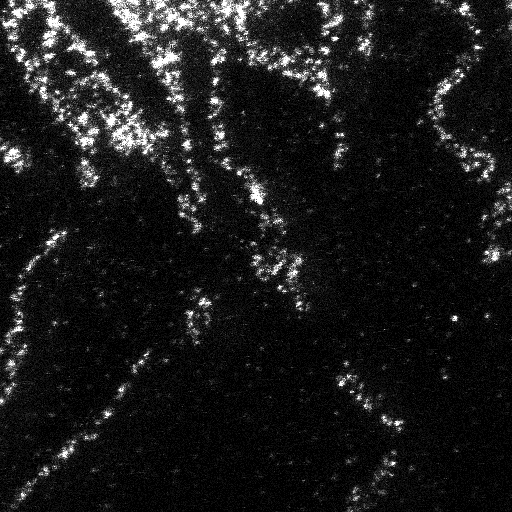
\includegraphics[width=0.095\linewidth]{images/micro512_1008} & 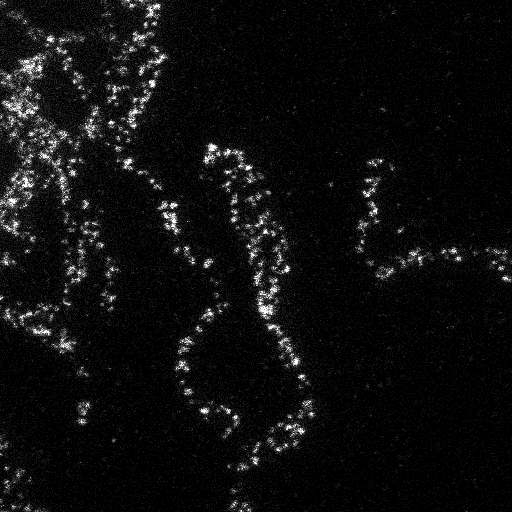
\includegraphics[width=0.095\linewidth]{images/micro512_1009} &
  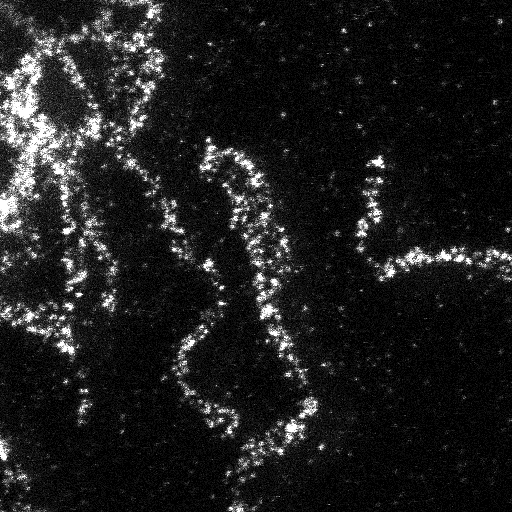
\includegraphics[width=0.095\linewidth]{images/micro512_1010} \\
    
\includegraphics[width=0.095\linewidth]{images/shapes512_1001}  & 
\includegraphics[width=0.095\linewidth]{images/shapes512_1002} &
  
\includegraphics[width=0.095\linewidth]{images/shapes512_1003} & 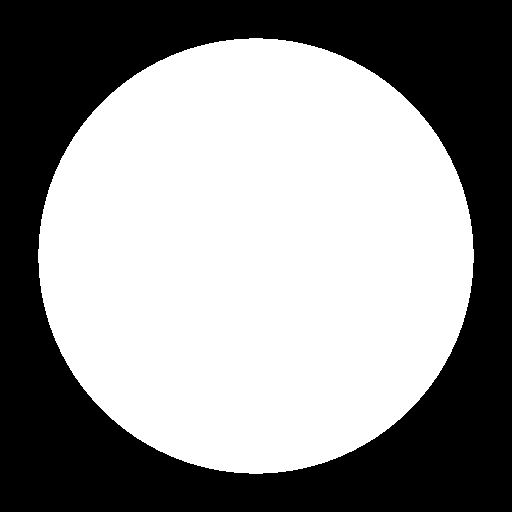
\includegraphics[width=0.095\linewidth]{images/shapes512_1004} &
  
\includegraphics[width=0.095\linewidth]{images/shapes512_1005} &
  
\includegraphics[width=0.095\linewidth]{images/shapes512_1006}  & 
\includegraphics[width=0.095\linewidth]{images/shapes512_1007} &
  
\includegraphics[width=0.095\linewidth]{images/shapes512_1008} & 
\includegraphics[width=0.095\linewidth]{images/shapes512_1009} &
  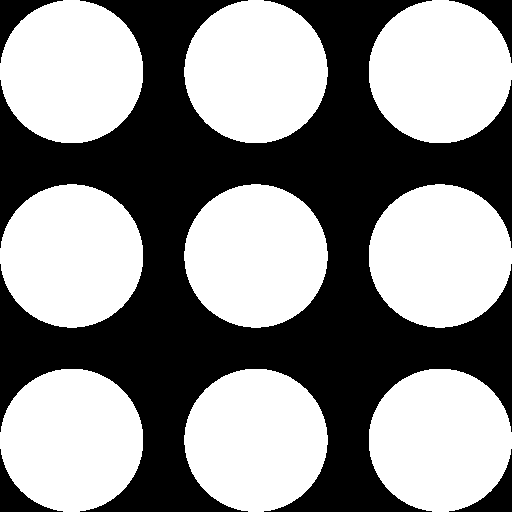
\includegraphics[width=0.095\linewidth]{images/shapes512_1010} \\
 \end{tabular}}
\caption{DOTmark benchmark: Classic, Microscopy, and Shapes images. \label{fig:dot}}
\end{figure}

\begin{table}[t!]
\caption{Comparison on $32 \times 32$ images. The runtime (in secs) is given as ``Mean (StdDev)''.
The gap to the optimum {\it opt} is computed as $\frac{UB-opt}{opt}\cdot 100$, where $UB$ is the upper bound computed by Sinkhorn's algorithm.
Each row reports the averages over 45 instances.
\label{tab:1}}
\centering
{\renewcommand{\arraystretch}{1.2}
\begin{tabular}{l|c|@{\hskip 0.3in}cr|@{\hskip 0.3in}cr|@{\hskip 0.3in}c|@{\hskip 0.3in}c}
      \multicolumn{1}{c}{}& \multicolumn{1}{c}{EMD\cite{Rubner98}} &  \multicolumn{4}{c}{Sinkhorn \cite{Cuturi2013}} & \multicolumn{1}{c}{Bipartite} & \multicolumn{1}{c}{$3$-partite} \\
	  \multicolumn{1}{c}{}& \multicolumn{1}{c}{}& \multicolumn{2}{c}{$\lambda=1$} & \multicolumn{2}{c}{$\lambda=1.5$} &  \multicolumn{1}{c}{}&  \\
	  \hline
Image Class & Runtime & Runtime & Gap & Runtime & Gap & Runtime & Runtime \\
\hline
Classic    & 24.0 (3.3) & 6.0 (0.5) & 17.3\% & 8.9 (0.7) & 9.1\%  & 0.54 (0.05) & {\bf 0.07 (0.01)}\\
Microscopy & 35.0 (3.3) & 3.5 (1.0) &  2.4\% & 5.3 (1.4) & 1.2\% & 0.55 (0.03) & {\bf 0.08 (0.01)}\\
Shapes     & 25.2 (5.3) & 1.6 (1.1) &  5.6\% & 2.5 (1.6) & 3.0\% & 0.50 (0.07) & {\bf 0.05 (0.01)}\\
 \hline\noalign{\smallskip}
 \multicolumn{8}{c}{} \\
 \end{tabular}}
\centering
{\renewcommand{\arraystretch}{1.2}
\setlength{\tabcolsep}{5pt}
\begin{tabular}{l|cr|@{\hskip 0.2in}cr|@{\hskip 0.2in}cr|@{\hskip 0.2in}c}
  \multicolumn{1}{c}{}    & \multicolumn{6}{c}{Improved Sinkhorn \cite{Solomon2015}} & \multicolumn{1}{c}{$3$-partite} \\
	\multicolumn{1}{c}{}  & \multicolumn{2}{c}{$\lambda=1$} & \multicolumn{2}{c}{$\lambda=1.25$}  & \multicolumn{2}{c}{$\lambda=1.5$}  &  \\
\hline
Image Class     & Runtime           & Gap       & Runtime           & Gap       & Runtime           & Gap       &   Runtime \\
\hline
 CauchyDensity	&	0.22	(0.15)	&	2.8\%	&	0.33	(0.23)	&	2.0\%	&	0.41	(0.28)	&	1.5\%	&	{\bf 0.07	(0.01)}	\\
 Classic		&	0.20	(0.01)	&	17.3\%	&	0.31	(0.02)	&	12.4\%	&	0.39	(0.03)	&	9.1\%	&	{\bf 0.07	(0.01)}	\\
 GRFmoderate	&	0.19	(0.01)	&	12.6\%	&	0.29	(0.02)	&	9.0\%	&	0.37	(0.03)	&	6.6\%	&	{\bf 0.07	(0.01)}	\\
 GRFrough		&	0.19	(0.01)	&	58.7\%	&	0.29	(0.01)	&	42.1\%	&	0.38	(0.02)	&	31.0\%	&	{\bf 0.05	(0.01)}	\\
 GRFsmooth		&	0.20	(0.02)	&	4.3\%	&	0.30	(0.04)	&	3.1\%	&	0.38	(0.04)	&	2.2\%	&	{\bf 0.08	(0.01)}	\\
 LogGRF			&	0.22	(0.05)	&	1.3\%	&	0.32	(0.08)	&	0.9\%	&	0.40	(0.13)	&	0.7\%	&	{\bf 0.08	(0.01)}	\\
 LogitGRF		&	0.22	(0.02)	&	4.7\%	&	0.33	(0.03)	&	3.3\%	&	0.42	(0.04)	&	2.5\%	&	{\bf 0.07	(0.02)}	\\
 Microscopy 	&	0.18	(0.03)	&	2.4\%	&	0.27	(0.04)	&	1.7\%	&	0.34	(0.05)	&	1.2\%	&	{\bf 0.08	(0.02)}	\\
 Shapes			&	0.11	(0.04)	&	5.6\%	&	0.16	(0.06)	&	4.0\%	&	0.20	(0.07)	&	3.0\%	&	{\bf 0.05	(0.01)}	\\
 WhiteNoise		&	0.18	(0.01)	&	76.3\%	&	0.28	(0.01)	&	53.8\%	&	0.37	(0.02)	&	39.2\%	&	{\bf 0.04	(0.00)}	\\
\hline\noalign{\smallskip}
 \end{tabular}}
\end{table}



\small
\bibliographystyle{plain}      % mathematics and physical sciences
\bibliography{references}   % name your BibTeX data base
\end{multicols}
\end{document}